\chapter{Introduction}


\section{Introduction to Thesis}
%\MT{Statements about historical background of quantum optics/quantum information/quantum cryptography}

This Thesis consists of two halves. In the first half, we consider several related cryptographic protocols which securely perform the tasks of Quantum Digital Signatures (QDS) and Quantum Secret Sharing (QSS). Our goals here are, firstly: to remove an assumption of secure quantum channels from continuous-variable (CV) QDS, and provide a security proof when an eavesdropping attack is permitted; and secondly: to demonstrate that several CV quantum cryptographic protocols may be performed over identical hardware setups, while the hardware at the quantum level is agnostic to the protocol being implemented. This so-called ``agile'' approach illustrates a translation of cryptographic agility from classical (conventional) cryptography to quantum cryptography, and allows for a move towards secure and practical quantum cryptosystems which can perform multiple tasks.

In the second half we consider the task of quantum state generation. We design and analyse a system which is capable to deterministically produce highly non-classical states at the output, from a coherent state input. Using methods from the fields of nonlinear pulse propagation in fibers and of open quantum systems, we analytically and numerically analyse a large multimode system and reduce it, step-by-step, to a single-mode system which is much more numerically tangible. The device, which we denote PhoG (\underline{Pho}ton \underline{G}un), will soon be implemented in a waveguide array structure and will provide a practical and cheap source of nonclassicality for quantum enhanced imaging and metrology, and may even improve the performance of quantum cryptographic systems. 

The two halves of this thesis can be interpreted as studying different aspects of quantum networked systems, in which both the individual systems, and the geometry of coupling between them, play an important role. The first half considers quantum communications networks and cryptographic tasks which are inherently multipartite. By studying the simplest networks of just three players (in two different configurations) we move towards cryptosystems which can be implemented entirely agnostic to the network structure. In the second half we consider large structures of waveguide arrays, where the dynamics are intimately connected to the underlying geometry. We focus on quantum correlation flow and coherent signal propagation in this device of connected bosonic modes, which will soon be created in laser-inscribed waveguides.

\subsection*{Detailed overview}

This Thesis is structured as follows. In the remainder of this Chapter we will introduce and outline several of the theoretical and analytical tools which we make extensive use of in the rest of the Thesis. We will show how the electromagnetic field may be quantized, discuss several common and useful quantum states of the field, and examine one method for their description and visualization. In Chapter~\ref{chapter:crypto_intro} we outline some of the developments in conventional cryptography which underpin our modern communications infrastructure, and discuss how two cryptographic tasks -- digital signatures and secret sharing -- may be translated to the quantum realm. In particular we will look at several recent and historic attempts to build such quantum protocols.

\paragraph{Part One:} In Chapter~\ref{chapter:qds} we introduce our own QDS protocol, and prove its security against several classes of attack. We show that ours is the first CV QDS protocol to allow for an eavesdropper on the channels, and we show that despite this we attain very short signature lengths over practical distances. In Chapter~\ref{chapter:qss} we introduce our QSS protocol, prove its security, and analyse its performance. Crucially, unlike several recent QSS protocols, our protocol does not require generation and distribution of large-scale entangled states, nor does it require dedicated hardware for a sequential ``round-robin'' style of approach. In the last chapter of Part One, Chapter~\ref{chapter:aqc}, we introduce and discuss the concept of quantum cryptographic agility, and demonstrate how it may apply to the protocols discussed in earlier chapters. We additionally introduce a new QDS protocol which runs in a modified configuration, and discuss how a quantum key distribution (QKD) protocol which already exists in the literature may be adopted into our agile system. We finish with a figure-of-merit graph which demonstrates that our QDS scheme, in addition to being practical and compatible with commercial telecommunications hardware, is also the fastest QDS protocol over comparable distances. 

\paragraph{Part Two:} In Chapter~\ref{chapter:phog} we motivate and introduce the PhoG device which will be the focus of the second half of this Thesis. We demonstrate that dissipation, far from being a hindrance to the desired evolution of our quantum system, is actually an asset and the main driver towards target nonclassicality. We introduce an exotic form of dissipation, called Nonlinear Coherent Loss, and show that in the ideal limit it will deterministically lead to single photons at the output. We then introduce progressively more complex models involving additional bosonic system modes, and demonstrate that a realistic full multi-mode model of the system can be used to effectively simulate the Nonlinear Coherent Loss decay channel. Finally, we end the chapter by demonstrating that in addition to generating highly sub-Poissonian states, a slight modification to the PhoG device will lead to generation of entanglement at the output.

\paragraph{Part Three:} We finish the Thesis with the inclusion of several appendices containing results which are used at multiple points throughout the Thesis.  Appendix~\ref{appendix:noisy_perr} contains results describing the output state of a channel in which an initial coherent state is mixed with thermal noise. This result is used multiple times throughout Part One. Appendix~\ref{appendix:crypto_numerical_methods} contains the forms of quantum states which are used under various channel attacks in Chapter~\ref{chapter:qds}, and a description of how the states may be numerically modelled. Appendix~\ref{appendix:qds_larger_alphabets} contains a generalization of the QDS protocol from Chapter~\ref{chapter:qds} to allow for larger alphabets of coherent states.  Appendix~\ref{appendix:adiabatic_elimination} provides a tool which is used multiple times in Chapter~\ref{chapter:phog} to reduce the complexity of a model by effectively ignoring a mode which reaches its steady state much quicker than the typical decay time of the system. Finally, in Appendix~\ref{appendix:phog_numerical_methods} we describe several numerical methods which may be applied to model the PhoG device. We compare them for speed, memory usage and accuracy, and then explicitly display several systems of coupled differential equations which approximate the PhoG device. 

\section{Introduction to Quantum Physics}

In this Thesis we are primarily interested in the quantum properties of single- or few- mode states of light. This Chapter will serve as a short introduction to several of the key concepts which we deal with, and some of their main properties. We first introduce the state vector and density matrix formalisms for description of quantum modes, in which the physical state is completely described by sums and outer products of vectors chosen from a countably infinite Hilbert space. We introduce single-mode operators and several single-mode states, and visualise them using a quantum analogue of a classical phase-space probability distribution known as the Wigner function. Multi-mode quantum states are introduced as states on larger vector spaces which are formed via a tensor product operation.

We introduce a third description of the quantum state which captures the second moments (co-variances) of multi-mode states, the so-called covariance matrix. This allows for a complete description of properties of a state which is Gaussian in phase-space, otherwise it offers a partial description which is nonetheless useful. 

Evolution of the quantum state is described by the von Neumann equation (no dissipation) or the Lindblad master equation (including dissipation). The latter allows for us to model the dynamics of a few modes chosen from much larger multi-mode system, provided that the two are weakly coupled and the larger system (environment/reservoir) is effectively unchanged by the system evolution. 

Finally, we display several selected entropic and probabilistic relations and quantities which we use in this Thesis. In particular, the notion of conditional probability, and the intimately related Bayes' theorem, will prove useful both as helpful quantities in their own right, and as foundational building blocks for conditional classical and quantum entropies. 





\FloatBarrier
\subsection{State vectors and density matrices}\label{sec:intro_state_vectors}
An ideal quantum state is denoted in the Dirac notation by $\ket{\psi}$. This state has been perfectly prepared with no noise, loss, or additional uncertainty due to the preparation. The $\ket{\psi}$ is a vector living in a vector space denoted $\mathcal{H}$, which we call a Hilbert space. The space has dimension $\dims$, typically taken to be countably infinite, but there will be several points in this Thesis where we consider a finite $\dims$.

Since $\ket{\psi}$ is a vector it can be written in terms of a set $\left\{\ket{e_j}\right\}$ of basis vectors,
\begin{equation}
\ket{\psi} = \sum_j c_j \ket{e_j},
\end{equation}
where the number of basis vectors typically equals $\dims$. 

The state $\ket{\psi}$ should be normalized, that is
\begin{equation}
\ip{\psi} = 1.
\end{equation}
The notation $\ip{\psi}$ means 
\begin{equation}
\sum_j \left|c_j\right|^2.
\end{equation}

\noindent We define an eigenstate of an arbitrary quantum operator $\hat{r}$ to be the state $\ket{r}$ such that
\begin{equation}
\hat{r} \ket{r} = r \ket{r}
\end{equation}
with eigenvalue $r \in \mathbb{C}$.

The basis we choose for vector $\ket{\psi}$ is not unique and we may similarly have expanded $\ket{\psi}$ in terms of eigenstates of $\hat{r}$, as
\begin{equation}
\ket{\psi} = \sum_j \ket{r}\ip{r}{\psi},
\end{equation}
where the $\ip{r}{\psi} \in \mathbb{C}$ is such that its square modulus $\left|\ip{r}{\psi}\right|^2$ is the probability that a measurement of $r$ on $\ket{\psi}$ will give outcome $r$.

For convenience any basis vectors we use are chosen to be orthonormal, that is
\begin{equation}
\ip{\hat{e}_j}{\hat{e}_k} = \delta_{j, k}
\end{equation}
where $\delta_{j, k}$ is the Kronecker $\delta$ function.

The fact that a state $\ket{\psi}$ may be written as a sum of basis vectors corresponding to different possible measurement outcomes is a curious one, and is a key feature of quantum mechanics known as the \emph{superposition principle}. A superposition state is one of the form
\begin{equation}\label{eqn:intro_superposition}
\ket{\psi} = \frac{\ket{0} + \ket{1}}{\sqrt{2}}
\end{equation}
where the constant factor $1/\sqrt{2}$ ensures normalization. We have chosen an abstract orthonormal basis set $\left\{ \ket{0}, \ket{1}\right\}$, and here $\dims=2$. The superposition state possesses a fundamental uncertainty about its measurement outcomes, that is to say, if many identical copies of $\ket{\psi}$ are created, and on each copy a measurement which distinguishes between $\ket{0}$ and $\ket{1}$ is performed, then the measurement will output $0$ half of the time, and $1$ the other half of the time. If, however, we are able to perform a measurement which distinguishes between $\left(\ket{0} \pm \ket{1}\right)/\sqrt{2}$, then we will find the output $\left(\ket{0} + \ket{1}\right)/\sqrt{2}$ $100\%$ of the time. This is markedly different from a statistical mixture, involving classical ignorance about whether the state is $\ket{0}$ or $\ket{1}$. 


% Such uncertainty is intrinsic to quantum mechanics and is unavoidable. However, unlike a classical uncertainty which one aims to reduce, this quantum uncertainty is highly desirable and forms the basis for many applications of quantum states.

The density operator corresponding to a quantum state is
\begin{equation}
\hat{\rho} = \sum_{i, j} p_{i, j} \dyad{i}{j}
\end{equation}
where $\bra{i} \in \mathcal{H}^*$ is dual to $\ket{i}$ ($\mathcal{H}^*$ is the dual space to $\mathcal{H}$). %The matrix $p_{i, j}$ is referred to as the density matrix, though we shall often use the terms \emph{density operator} and \emph{density matrix} interchangably. As such, we will often neglect the hat above $\hat{\rho}$, and simply write $\rho$.
Since We shall often use the terms \emph{density operator} and \emph{density matrix} interchangeably.

Any state vector $\ket{\psi}$ can be described as a density operator. For example, the state $\ket{\psi}$ in Eq.~\ref{eqn:intro_superposition} may equivalently be described as 
\begin{equation}
\rho_\psi = \dyad{\psi}{\psi} = \frac{1}{2} \left(\dyad{0}{0} + \dyad{0}{1} + \dyad{1}{0} + \dyad{1}{1} \right).
\end{equation}
However, there are density operators which do not correspond to a state vector. For example, there exists no vector $\ket{\phi}$ such that
\begin{equation}\label{eqn:intro_mixture}
\rho_{\varphi} := \frac{\dyad{0}{0} + \dyad{1}{1}}{2} = \dyad{\phi}.
\end{equation}
The density operator formalism may be interpreted as encoding two distinct forms of uncertainty: quantum and classical. The quantum uncertainty arises from states which may be written as superposition state vectors, while the classical uncertainty arises from states which cannot. We refer to the first type of summation as superposition, and the second type of summation as classical mixing (or a statistical mixture). The classical mixing represents classical uncertainty about which state the system is in, and may in principle be removed by building better equipment.

In the $\left\{\ket{0}, \ket{1}\right\}$ basis, these states $\rho_\psi$ and $\rho_\varphi$ may be written as
\begin{equation}
\rho_\psi = \frac{1}{2}\pmqty{1 & 1 \\ 1 & 1} \qq{and} \rho_\varphi = \frac{1}{2}\pmqty{1 & 0 \\ 0  & 1}.
\end{equation}

\noindent The quantum nature of a state $\rho$ is therefore intimately connected to the off-diagonal elements of its density matrix. These off-diagonal elements may be referred to as \emph{coherences}. The density matrix $\rho$ will be our primary tool for describing a quantum state in this Thesis.

%\FloatBarrier
%\subsection{Quantum optics}
%\MT{Add some chat about quantizing the field, and lead up to introduction of $\hat{a}$.}


\FloatBarrier
\subsection{Introduction to quantum optics}

In the absence of currents or charge, classical electromagnetic fields obey Maxwell's equations:

\begin{equation}
\nabla \cdot \bm{B} =0,\qq{} \nabla \times \bm{E} = - \frac{\partial \bm{B}}{\partial t},\qq{} \nabla \cdot \bm{D} = 0 \qq{and} \nabla \times \bm{H} = \frac{\partial \bm{D}}{\partial t}.
\end{equation}

\noindent We may quantize these electric and magnetic fields by replacing the vectors $\bm{B}, \bm{E}, \bm{D}, \bm{H}$ with the corresponding operators $\hat{\bm{B}}, \hat{\bm{E}}, \hat{\bm{D}}, \hat{\bm{H}}$, and imposing that the classical fields should be regarded as expected values of these quantum operators:

\begin{equation}
\bm{E} = \ev{\hat{\bm{E}}}{\psi} \qq{etc.}
\end{equation}

\noindent By analogy with the classical vector potential, let us introduce the quantum vector potential $\hat{\bm{A}}$, and impose
\begin{equation}
\hat{\bm{E}} = - \frac{\partial \hat{\bm{A}}}{\partial t}, \qq{}  \hat{\bm{B}} = \nabla \times \hat{\bm{A}}, \qq{and} \nabla \cdot \hat{\bm{A}} = 0.
\end{equation}
As in classical electromagnetism, the first two of these requirements automatically imply that the first two of Maxwell's equations are satisfied, while the third requirement (``coulomb gauge'') is merely a convenient choice which immediately satisfies the third Maxwell equation\footnote{Since light in linear media behaves as $\hat{\bm{D}} = \epsilon_0 \epsilon \hat{\bm{E}}$, where $\epsilon_0$ is the vacuum permittivity and $\epsilon$ is the electric permittivity of the medium in question. The other ``constitutive equation'' is $\hat{\bm{H}} = \mu_0^{-1} \mu^{-1} \hat{\bm{B}}$, for medium permeability $\mu$ and vacuum permeability $\mu_0$.}. The final Maxwell equation is then equivalent to the following wave equation

\begin{equation}\label{eqn:intro_wave}
\epsilon^{-1} \mu^{-1} \nabla \times \nabla \times \hat{\bm{A}} = - c^{-2} \frac{\partial^2 \hat{\bm{A}}}{\partial t^2}.
\end{equation}

\noindent These equations contain all of the same information as Maxwell's equations, just involving the quantized vector potential. This $\hat{\bm{A}}$ contains all information about our light wave. The Hamiltonian of our electromagnetic field takes the same form as the classical total energy, i.e.
\begin{equation}\label{eqn:intro_hamiltonian}
\hat{H} = \int_V \Diff3 V \; \frac{\hat{\bm{E}} \cdot \hat{\bm{D}} + \hat{\bm{B}} \cdot \hat{\bm{H}}}{2}.
\end{equation}


\noindent The electromagnetic wave equation, Eq.~\ref{eqn:intro_wave} is a linear differential equation, and so obeys the superposition principle. Let us define a set of monochromatic classical waves
\begin{equation}
\bm{A}_j\left(\overrightarrow{r}, t\right) = \bm{A}_j\left(\overrightarrow{r}\right) \exp^{-i \omega_j t}
\end{equation}
oscillating at frequency $\omega_j$. We have assumed that the temporal and spatial aspects of the wave can be separated, and let the vector $\bm{A}_j\left(\overrightarrow{r}\right)$ contain all spatial information. %The $\bm{A}_j$ form an orthonormal basis set.
Let us expand the quantum vector potential $\hat{\bm{A}}$ as
\begin{equation}
\hat{\bm{A}}\left(\overrightarrow{r}, t\right) = \sum_k \left[ \bm{A}_j\left(\overrightarrow{r}, t\right) \hat{a}_j + \bm{A}_j^* \left(\overrightarrow{r}, t\right) \hat{a}_j^\dagger\right]
\end{equation}
where we have introduced single-mode quantum operators $\hat{a}_j, \hat{a}_j^\dagger$.

Substituting this $\hat{\bm{A}}\left(\overrightarrow{r}, t\right)$, expanded in a basis of monochromatic waves, into the Hamiltonian Eq.~\ref{eqn:intro_hamiltonian}, we arrive at
\begin{equation}\label{eqn:intro_hamiltonian_2}
\hat{H} = \sum_j \hbar \omega_j \left( \hat{a}_j^\dagger \hat{a}_j + \frac{1}{2}\right),
\end{equation}
where we have used the commutator $\left[ \hat{a}_j \hat{a}_k^\dagger \right] = \delta_{j, k}$. We are thus led to identify the $\hat{a}_j, \hat{a}_j^\dagger$ as the raising and lowering operators of a simple harmonic oscillator which obeys the Hamiltonian Eq.~\ref{eqn:intro_hamiltonian_2}. 

We have effectively split the full quantum description of light into two parts, classical and quantum. The classical quantities $\bm{A}_j\left(\overrightarrow{r}, t\right)$ fully describe all wave properties of the light, while the quantum operators $\hat{a}_j$ describe the quanta present in a single mode. For this Thesis we will focus on these quantum systems and ignore the wave nature of light. That is to say, we will regard the mode operators $\hat{a}_j$ as accurately describing the full system, irrelevant of its classical properties. This proves to be a helpful distinction as it allows for us to make general quantum statements which are true for any bosonic system of quantum modes, regardless of their physical implementation.

In Sec.~\ref{sec:phog_outlook} we will briefly return to the classical $\bm{A}\left(\overrightarrow{r}, t\right)$ in a $1+1$D system (one spatial dimension plus time). The $A\left(z, t\right)$ are discussed there in the context of light pulse propagation in waveguides where, with physical implementation in mind, we must pay great attention to the wave properties. We discuss there some methods to efficiently model such classical behaviour, and then mention as outlook several strategies which may be used to model the full propagation of a quantum pulse, taking into account both classical and quantum effects.

For a more detailed discussion of the derivation presented here, we refer the reader to the textbooks Refs.~\cite{Leonhardt2010, Walls_Millburn_Textbook, Gerry_Knight_Textbook}.


\FloatBarrier
\subsection{Single-mode operators}
The bosonic operators $\hat{a}, \hat{a}^\dagger$ create and destroy a quantum of energy in the light mode. These operators obey the bosonic commutation relation
\begin{equation}
\left[ \hat{a}, \hat{a}^\dagger \right] = 1,
\end{equation}
and are crucial for modelling the quantum properties of our light. 

We define the photon-number operator $\hat{n}$ as 
\begin{equation}
\hat{n} = \hat{a}^\dagger \hat{a},
\end{equation}
which counts the number of photons in our mode.

We may construct the following two operators

\begin{equation}\label{eqn:intro_quadrature}
\hat{q} = \sqrt{\frac{\hbar}{2 \omega}}\left(\hat{a}^\dagger + \hat{a}\right) \qq{and} \hat{p} = i \sqrt{\frac{\hbar \omega}{2}}\left(\hat{a}^\dagger - \hat{a}\right)
\end{equation}
which are known as the ``quadrature operators'', and can be shown to obey the commutator
\begin{equation}\label{eqn:intro_quadrature_commutator}
\left[\hat{q}, \hat{p}\right] = i \hbar.
\end{equation}
The quadrature operators $\hat{q}$ and $\hat{p}$ correspond to field amplitudes which are $\pi/2$ out of phase with each other. The annihilation operator can then be written
\begin{equation}
\hat{a} = \frac{1}{\sqrt{2 \hbar \omega}} \left(\omega\hat{q} + i \hat{p}\right).
\end{equation}

\noindent The quadrature operator for a general quadrature $\hat{q}_\theta$ is given by
\begin{equation}
\hat{q}_\theta = \hat{q} \cos\theta  + \hat{p} \sin\theta ,
\end{equation}
and the operators $\hat{q}$, $\hat{p}$ are recovered as special cases with $\theta = 0$ and $\pi/2$, respectively. The quadrature operators $\hat{q}, \hat{p}$ may be used to write the well known Heisenberg uncertainty principle as
\begin{equation}\label{eqn:intro_uncertainty}
\text{Var}\left(\hat{q}\right)\text{Var}\left(\hat{p}\right) \ge \hbar^2/4, %note that this is 1/4 not 1/2, due to using variances (not standard deviations) on the LHS. c.f. Ulf eq 3.80 p54
\end{equation} 
where the variances in a general quantum state $\ket{\psi}$ are defined as
\begin{align}
\text{Var}\left(\hat{q}\right) &= \mel{\psi}{\hat{q}^2}{\psi} - \mel{\psi}{\hat{q}}{\psi}^2, \notag \\
\text{Var}\left(\hat{p}\right) &= \mel{\psi}{\hat{p}^2}{\psi} - \mel{\psi}{\hat{p}}{\psi}^2.
\end{align}
The uncertainty principle Eq.~\ref{eqn:intro_uncertainty} implies that we cannot simultaneously measure $\hat{q}$ and $\hat{p}$ with arbitrary precision - in other words $q$ and $p$ are conjugate variables.

The $\mel{\psi}{\hat{q}}{\psi}$ denote the expectation value of $\hat{q}$ in state $\ket{\psi}$. We may equivalently write this as $\ev{\hat{q}}_\psi$, or simply just $\ev{\hat{q}}$ when the corresponding state is obvious. The expectation value of an operator corresponds to the average measurement outcome when many measurements of that operator is performed on the given state.

The commutator Eq.~\ref{eqn:intro_quadrature_commutator} is equivalent to the commutator between operators which describe position and momentum of a quantum particle, and so we identify $\hat{q}$ as the position operator and $\hat{p}$ as the momentum operator (thus corroborating Eq.~\ref{eqn:intro_uncertainty}). Indeed, it is easy to show from the definitions that
\begin{equation}
\hat{H} = \omega^2 \frac{\hat{q}^2}{2} + \frac{\hat{p}^2}{2} = \hbar \omega \left(\hat{n} + \frac{1}{2}\right) ,
\end{equation}
the middle terms of which describes the energy of a simple harmonic oscillator in what follows we will set $\hbar=1$ for convenience.





\FloatBarrier
\subsection{Wigner function}
An equivalent way to describe the quantum state $\rho$ is to use a (\emph{quasi})-probability distribution known as the Wigner function. The Wigner function, $W\left(q, p\right)$, allows operator expectation values to be calculated using an averaging method similar to classical mechanics in phase space. %For this reason, we desire $W\left(q, p\right)$ to behave analogously to a joint probability distribution, by analogy with a classical phase space picture in which the system is described in terms of position and momentum. We thus introduce a \emph{quantum} phase space. 

One immediate observation is that a \emph{quantum phase space} must behave qualitatively very differently to the classical one. Because of Heisenberg's principle, we cannot accurately define a joint probability distribution of position $q$ and momentum $p$ as this would require precise knowledge of both quantities. This leads to interesting behaviours of the phase space ``probability'' distribution, such as becoming negative (for Wigner functions) or highly singular (for ``$P$-functions''). Indeed, one may even measure the ``quantumness'' of a given state by checking for these properties.

We define the Wigner function corresponding to density operator $\hat{\rho}$ as \cite{Leonhardt2010}

\begin{equation}\label{eqn:intro_wigners_formula}
W\left(q, p\right) = \frac{1}{2 \pi} \int\limits_{-\infty}^{\infty} \mathrm{d}x \; \exp\left(i p x\right) \mel{q - \frac{x}{2}}{\hat{\rho}}{q + \frac{x}{2}}.
\end{equation}

\noindent The marginal distributions of $W$ are genuine probability distributions, and are given by tracing out the conjugate quadrature:

\begin{equation}
\text{P}\left(q\right) = \int\limits_{-\infty}^\infty \mathrm{d}p \; W\left(q, p\right) \qq{and} \text{P}\left(p\right) = \int\limits_{-\infty}^\infty \mathrm{d}q \; W\left(q, p\right).
\end{equation}

\noindent A useful feature of the Wigner function is that traces over operators may be calculated as

\begin{equation}\label{eqn:wigner_overlap}
\tr\left[\hat{O}_1 \hat{O}_2\right] = 2\pi \int\limits_{-\infty}^\infty \int\limits_{-\infty}^{\infty} \mathrm{d}q \; \mathrm{d}p \; W_1\left(q, p\right) W_2\left(q, p\right)
\end{equation}
where $W_i\left(q, p\right)$ is the Wigner function corresponding to operator $\hat{O}_i$. Operator expectation values with respect a given state $\hat{\rho}$ may be calculated using Eq.~\ref{eqn:wigner_overlap}. 

The Heisenberg uncertainty relation further expresses itself in the Wigner function picture by imposing a minimum area which a quantum state must occupy. In the following sections we will see some examples of quantum states and their corresponding Wigner functions. In all plots of Wigner functions, the colour blue denotes $W\left(q, p\right) >0$ while red denotes $W \left(q, p\right) <0$. Negativity (red, in this Thesis) in the Wigner function is a clear sign that the underlying state is nonclassical\footnote{Indeed, the only pure quantum states with non-negative Wigner functions are those with Gaussian Wigner function, i.e. the Glauber coherent states and the quadrature squeezed states.}.



Finally, we must note that the Wigner function is not the only quasi-probability distribution which one could define on the phase space, and because in general quantum operators do not commute there are multiple ways to consistently define a phase space description. Other common quasi-probability distributions are: the Hussimi $Q$ function \cite{Husimi1940}, which is intimately related to heterodyne measurement; Glauber-Sudarshan \cite{Glauber1963} $P$ function, which is often used to describe mixtures of coherent states and becomes highly singular in all other cases; and the positive-$P$ function, which is a generalization to the $P$ function and is defined to be non-diagonal in the coherent state basis, and which allows quantum effects such as squeezing to be described \cite{Walls_Millburn_Textbook}. One may also use these quasi-probability distributions to predict dynamics of the system using a Fokker-Planck diffusion equation \cite{Carmichael1999}, analogously to a classical stochastic process.

We use the Wigner function in Appendix~\ref{appendix:noisy_perr} to simplify a calculation which is analytically difficult in the density matrix picture, and the Wigner functions offer an excellent visualization tool in the following few sections.


\FloatBarrier
\subsection{Fock states}
Fock states (also called photon-number states) are defined as eigenstates of the photon-number operator $\hat{n} = \hat{a}^\dagger \hat{a}$:
\begin{equation}
\hat{n} \ket{n} = n \ket{n}.
\end{equation}
In other words, $\hat{n}$ measures the number of photons in $\ket{n}$. The states have perfectly defined photon-number and find many applications in quantum information processing \cite{Bennett1984, Adami1999}. The creation and annihilation operators $\hat{a}^\dagger, \hat{a}$ act on $\ket{n}$ as 
\begin{align*}
\hat{a}\ket{n} &= \sqrt{n}\ket{n-1}, \\
\hat{a}^\dagger \ket{n} &= \sqrt{n+1} \ket{n=1}.
\end{align*}
The Fock states form an orthogonal basis for $\mathcal{H}$:
\begin{equation}
\ip{m}{n} = \delta_{n, m},
\end{equation}
and so we will often seek an expansion of other states in the Fock-state basis. In particular, our density matrix $\rho$ is written in a Fock state expansion as
\begin{equation}
\rho_{m, n} = \mel{m}{\hat{\rho}}{n}.
\end{equation}

\noindent Wigner functions corresponding to some example Fock states are displayed in Fig.~\ref{fig:intro_fock_wigner}.



\begin{figure}[htp]
\centering
\captionsetup{width=0.8\linewidth}
	\begin{subfigure}{0.49\linewidth}
		\centering
		\includegraphics[draft=false, width=\linewidth]{introduction/fock_wigner_1}
	\end{subfigure}
	\begin{subfigure}{0.49\linewidth}
		\centering
		\includegraphics[draft=false, width=\linewidth]{introduction/fock_wigner_2}
	\end{subfigure}
\caption{\label{fig:intro_fock_wigner} Wigner functions for Fock states $\ket{1}$ and $\ket{2}$. Blue signifies that the Wigner function is positive, while red signifies that the Wigner function is negative. }
\end{figure}



\FloatBarrier
\subsection{Quadrature states}
We define the eigenstates of quadrature operators $\hat{q}$ and $\hat{p}$ as
\begin{equation}\label{eqn:intro_quadrature_state}
\hat{q}\ket{q} = q \ket{q} \qq{and} \hat{p}\ket{p} = p \ket{p}.
\end{equation}
These $\ket{q}, \ket{p}$ are known as quadrature states. Although they are not normalizable, the quadrature states are a useful tool in quantum optics. For example, we will use them to describe ideal homodyne detection, Sec.~\ref{sec:intro_homodyne}, and are also required for the definition of the Wigner function in Eq.~\ref{eqn:intro_wigners_formula}.


\FloatBarrier
\subsection{Coherent states}
Coherent states\footnote{Also known as Glauber coherent states \cite{Glauber1963}.} are among the most important quantum states which we discuss in this Thesis. The coherent state $\ket{\alpha}$ is defined as the eigenstate of annihilation operator $\hat{a}$:
\begin{equation}
\hat{a}\ket{\alpha} = \alpha \ket{\alpha}.
\end{equation}
This coherent state has amplitude $\alpha \in \mathbb{C}$, and we display an example of a coherent state Wigner function in Fig.~\ref{fig:intro_coherent_wigner}. It can be shown that the area occupied by the coherent state is the smallest allowable area of phase space for a Wigner function to cover. In other words, the coherent state saturates the Heisenberg bound and is a minimum uncertainty state.%, possessing the same uncertainty in $q$ and $p$ as the vacuum state.

\begin{figure}[htp]
\centering
\captionsetup{width=0.8\linewidth}
\includegraphics[draft=false, width=0.5\linewidth]{introduction/coherent}
\caption{\label{fig:intro_coherent_wigner} Wigner function for coherent state $\ket{\alpha}$ with $\alpha = 1 + 1i$.}
\end{figure}

\noindent The coherent states are non-orthogonal:
\begin{equation}
\ip{\alpha}{\beta} = \exp\left(- \frac{\left|\alpha\right|^2}{2} - \frac{\left|\beta\right|^2}{2} + \alpha^* \beta \right),
\end{equation}
where $\alpha^*$ denotes the complex conjugate of $\alpha$, and so we will regularly make use of an expansion of $\ket{\alpha}$ in the orthogonal Fock basis:
\begin{equation}\label{eqn:intro_coherent_fock}
\ket{\alpha} = e^{-\frac{\left|\alpha\right|^2}{2}} \sum_{n=0} \frac{\alpha^n}{\sqrt{n!}} \ket{n}.
\end{equation}

\noindent In the first part of this Thesis we will consider several quantum cryptographic protocols involving distribution of coherent states. We will regularly use an alphabet of coherent states known as the QPSK (Quadrature Phase-Shift Keying) alphabet, 

\begin{equation}
\qq*{QPSK alphabet:} \left\{\ket{\alpha}, \ket{i \alpha}, \ket{- \alpha}, \ket{- i \alpha}\right\},
\end{equation}

\noindent and we display a mixture over the QPSK alphabet in Fig.~\ref{fig:qpsk}. We will not explicitly distinguish between whether we refer to the set of quantum states $\left\{\ket{\alpha}, \ket{i \alpha}, \ket{- \alpha}, \ket{- i \alpha}\right\}$ or the corresponding set of complex amplitudes $\left\{ \alpha, i \alpha, -\alpha, - i\alpha\right\}$, since it should always be obvious which is meant.

A special case of the coherent states, that with eigenvalue $0$,
\begin{equation}
\hat{a} \ket{0} = 0 \ket{0}.
\end{equation}
\noindent This state is known as the ``vacuum'' state, and is a special example of a quantum state, since $\ket{0}$ is also an eigenstate of $\hat{n}$, and is thus a Fock state\footnote{It can also be viewed as a thermal state with $\bar{n}=0$, c.f. Sec.~\ref{sec:intro_thermal}.} with a photon number $0$. The coherent state possesses the same uncertainty properties as the vacuum state.


\begin{figure}[htp]
\captionsetup{width=0.8\linewidth}
\centering
\begin{subfigure}[b]{0.49\linewidth}
\includegraphics[draft=false, width=\linewidth]{introduction/qpsk_1}
\caption{}
\end{subfigure}
\begin{subfigure}[b]{0.49\linewidth}
\includegraphics[draft=false, width=\linewidth]{introduction/qpsk_2}
\caption{}
\end{subfigure}
\caption{\label{fig:qpsk} The Wigner function for a mixture over the QPSK alphabet is a sum of individual Wigner functions for each of the coherent states. QPSK alphabet with (a) $\alpha=1.5$; (b) $\alpha=0.8$.}
\end{figure}

\begin{figure}[htp]
\captionsetup{width=0.8\linewidth}
\centering
\begin{subfigure}[b]{0.49\linewidth}
\includegraphics[draft=false, width=\linewidth]{introduction/8psk_1}
\caption{}
\end{subfigure}
\begin{subfigure}[b]{0.49\linewidth}
\includegraphics[draft=false, width=\linewidth]{introduction/8psk_2}
\caption{}
\end{subfigure}
\caption{\label{fig:intro_npsk} $N$PSK coherent state alphabet with $N=8$. (a) $\left|\alpha\right|$ = 1.5. (b) $\left|\alpha\right|$=0.8.}
\end{figure}

A generalization to QPSK is the so-called $N$PSK alphabet, in which $N$ coherent states are chosen. The states are again equally distributed around the origin of phase space, and we note that QPSK is the special case $N=4$. We display an example in Fig.~\ref{fig:intro_npsk}.



\FloatBarrier
\subsection{Thermal states}\label{sec:intro_thermal}

The thermal state is defined as
\begin{equation}\label{eqn:intro_thermal}
\rho_{\text{thermal}} = \left( 1 - e^{-\beta} \right) \sum_{n=0}^\infty e^{- n \beta} \dyad{n},
\end{equation}
with $\beta = \left( \hbar \omega \right)/\left(k_B T\right)$, reduced Planck's constant $\hbar$, angular frequency $\omega$, Boltzmann's constant $k_B$ and thermal equilibrium temperature $T$. As we see from the form of Eq.~\ref{eqn:intro_thermal}, the thermal state is a classical mixture of Fock states (c.f. Eq.~\ref{eqn:intro_mixture}). Typically we will parametrise the thermal state using the average thermal photon number $\bar{n}$, which is defined as 
\begin{equation}
\bar{n} = \frac{1}{e^\beta - 1},
\end{equation}
which measures the average number of photons in the thermal state. We display the Wigner function of a thermal state in Fig.~\ref{fig:thermal_state}, where we have also displayed the vacuum state variance, for comparison.


\begin{figure}[htp]
\captionsetup{width=0.8\linewidth}
\centering
\includegraphics[draft=false, width=0.49\linewidth]{introduction/thermal_state}
\caption{\label{fig:thermal_state} The thermal state Wigner function is Gaussian, with variance greater than the vacuum state variance, which is depicted in orange.}
\end{figure}

\FloatBarrier
\subsection{Squeezed states (quadrature)}

We have already encountered the Heisenberg relation, which imposes a minimum phase space area which a state can occupy. The coherent state was a minimum uncertainty state and so occupied the minimum possible area while possessing symmetry: $\text{Var}\left( \hat{q}\right) = \text{Var}\left(\hat{p}\right)$. Of course, it is possible to satisfy the Heisenberg relation while also taking $\Delta q \ne \Delta p$, and this is precisely what (quadrature) squeezed states do. We display some examples of quadrature squeezed states in Fig.~\ref{fig:intro_quadrature_squeezed_wigner}. In the limit of infinite squeezing one obtains quadrature states $\ket{q}$ and $\ket{p}$.

Quadrature squeezing is generated by application of the squeezing operator
\begin{equation}
\hat{S}\left(\zeta\right) = \exp \left(\frac{\zeta}{2} \left(\hat{a}^2 - \hat{a}^{\dagger 2}\right) \right),
\end{equation}

\noindent which may be realised, for example, by degenerate parametric amplification \cite{Boyd2008}.


\begin{figure}[htp]
\centering
\captionsetup{width=0.8\linewidth}
	\begin{subfigure}{0.49\linewidth}
		\centering
		\includegraphics[draft=false, width=\linewidth]{introduction/squeeze_1}
	\end{subfigure}
	\begin{subfigure}{0.49\linewidth}
		\centering
		\includegraphics[draft=false, width=\linewidth]{introduction/squeeze_2}
	\end{subfigure}
\caption{\label{fig:intro_quadrature_squeezed_wigner} Quadrature squeezed states. Squeezing operator $\hat{S}\left(\zeta\right)$ has been applied to vacuum. (a) $\zeta = 1.0$. (b) $\zeta = -1.0$. Orange circles denote vacuum variance. Squeezed states allow for reduced uncertainty in one quadrature, at the expense of increased uncertainty in the conjugate quadrature.}
\end{figure}

\FloatBarrier
\subsection{Squeezed states (photon-number)}
We have seen that the coherent state $\ket{\alpha}$ may be expanded in Fock basis as Eq.~\ref{eqn:intro_coherent_fock}. From this equation it may be shown that the photon-number distribution of $\ket{\alpha}$ is 
\begin{equation}
\mathcal{P}_n\left[\ket{\alpha}\right] = \left| \ip{n}{\alpha} \right|^2 = \frac{\left|\alpha\right|^{2n}}{n!} e^{-\left|\alpha\right|^2}
\end{equation}
which obeys Poissonian statistics, i.e. its mean is equal to its variance. The thermal state can be shown to possess super-Poissonian photon statistics, with variance larger than its  mean. Conversely, a sub-Poissonian state has reduced photon-number variance, with a variance smaller than its mean. The Fock state, with zero photon-number uncertainty, is the limiting example of a sub-Poissonian state.

In addition to the quadrature squeezing discussed above, in which the variance in one quadrature was reduced at the expense of the other, we may think of a photon-number squeezed state in which the photon-number variance is reduced, at the expense of an increase in the phase variance\footnote{Note that quantifying such a statement is tricky, and we refer the reader to Ref.~\cite{Barnett_red_book} for discussion.}. We display the Wigner function of a photon-number squeezed state in Fig.~\ref{fig:intro_photon_number_squeezed_wigner}.

\begin{figure}[htp]
\centering
\captionsetup{width=0.8\linewidth}
\includegraphics[draft=false, width=0.5\linewidth]{introduction/photon_number_squeezed}
\caption{\label{fig:intro_photon_number_squeezed_wigner} A photon-number squeezed state has reduced photon number uncertainty, at the expense of increased uncertainty in phase. In the limit of zero photon number uncertainty one obtains a Fock state, Fig.~\ref{fig:intro_fock_wigner}. This state displayed here is only slightly photon-number squeezed, but more closely represents a Fock state Wigner function than a quadrature squeezed state does. }
\end{figure}



\FloatBarrier
\subsection{Mixing, purity, and entanglement}
%I need this section in order to introduce multiple modes, and trace operation.

\subsubsection{Purity}
We have already seen in Sec.~\ref{sec:intro_state_vectors} that the density matrix $\rho$ can encode two types of uncertainty, quantum and classical. The quantum uncertainty is related to superpositions of basis states and is insurmountable, while the classical uncertainty represents ignorance of which quantum state was prepared, and can in principle always be reduced. A state possessing only the first type of ignorance may in general be written as
\begin{equation}\label{eqn:intro_rho_pure}
\rho = \dyad{\psi} \qq{with} \ket{\psi} = \sum_n c_n \ket{n}
\end{equation}
where without loss of generality we have used the Fock basis, and the $c_n$ are complex coefficients. We call the the state Eq.~\ref{eqn:intro_rho_pure} a ``pure'' state. Any state which is not pure is ``mixed''. A state with \emph{only} the second type of ignorance may in general be written as
\begin{equation}\label{eqn:intro_rho_fully_mixed}
\rho = \sum_n d_n \dyad{n}
\end{equation}
where without loss of generality we have used the Fock basis, and $d_n$ are real coefficients. The state Eq.~\ref{eqn:intro_rho_fully_mixed} only has diagonal elements in its density matrix, and if there are two or more nonzero $d_n$, then the state is fully mixed.

Given a density matrix $\rho$, it is time consuming and difficult to check by hand which of these forms it takes, and in most situations it will not fit neatly into either form. We therefore desire a function which will identify and quantify which type of ignorance the state possesses, and which may be easily computed on $\rho$. To do this, we first introduce the trace of $\rho$ as
\begin{equation}
\tr\left[\rho\right] := \sum_m \mel{m}{\rho}{m},
\end{equation}
where without loss of generality we have used the Fock basis, but we note that we may instead sum over any orthonormal basis for $\mathcal{H}$. By definition, the trace of a normalized state must be $1$. We introduce the notion of \emph{purity} of a quantum state as a measure of how close to Eq.~\ref{eqn:intro_rho_pure} our state is. This may be measured by
\begin{equation}\label{eqn:intro_purity}
\tr\left[ \rho^2 \right],
\end{equation}
which we will simply call the purity. It can easily be shown that state Eq.~\ref{eqn:intro_rho_pure} has purity $1$ while state Eq.~\ref{eqn:intro_rho_fully_mixed} has purity $0$.

\subsubsection{Entanglement}

Let us now turn to consider two-mode quantum states. We have already seen that a single-mode quantum state exists as a vector on Hilbert space $\mathcal{H}$. To describe two modes, we introduce an additional Hilbert space and write $\mathcal{H}_{tot} = \mathcal{H}_1 \otimes \mathcal{H}_2$, where $\mathcal{H}_{1,2}$ are Hilbert spaces of the individual modes, $\otimes$ represents the tensor-product, and $\mathcal{H}_{tot}$ is the total Hilbert space. We may tensor product any two single-mode quantum states together to form a state on $\mathcal{H}_{tot}$, for example
\begin{equation}\label{eqn:intro_separable_1}
\ket{\alpha}_1 \otimes \ket{n}_2
\end{equation}
represents a state on $\mathcal{H}_{tot}$, consisting of a coherent state with amplitude $\alpha$ on $\mathcal{H}_1$, and an $n$ photon Fock state on $\mathcal{H}_2$. For convenience we will often write $\ket{\alpha, n}$ instead of $\ket{\alpha}_1 \otimes \ket{n}_2$.

Now, there are many states which we can write in the form Eq.~\ref{eqn:intro_separable_1}. The general form of this type of ``product-state'' is
\begin{equation}
\rho_{\text{product}} = \dyad{\Psi} \qq{with} \ket{\Psi} = \ket{\psi}_1 \otimes \ket{\phi}_2.
\end{equation}
A general ``separable state'' may be written
\begin{equation}\label{eqn:intro_separable_2}
\rho_{\text{separable}} = \sum_{i, j} c_{i, j} \dyad{\psi_i}_1 \otimes \dyad{\phi_j}_2,
\end{equation}
called ``separable'' because the total two-mode state can be separated out into distinct single-mode density operators of modes $1$ and $2$ individually. The separable state may be interpreted as a classical mixture of product states.

Any state which cannot be written in the form Eq.~\ref{eqn:intro_separable_2} is known as a ``non-separable'' or ``entangled'' state. Entangled states cannot be written as a classical mixture over single-mode density operators, and so even full information about each individual mode is not sufficient to fully describe the total system. Such a remarkable feature is one of the key departures of the quantum world from the classical one, and entanglement is itself a fundamental resource to accomplish quantum tasks \cite{Horodecki2009b, Eisert2003}.

\subsubsection{Partial trace}
Let $\rho = \sum_{i, j, k, l} c_{i, j, k, l} \ket{i, j}\bra{k, l}$ be a general two-mode density operator. We define the partial trace over mode $1$ as
\begin{align*}
\tr_1\left[\rho\right] = \sum_n \bra{n}\rho\ket{n} = \sum_n \bra{n} \left[\sum_{i, j, k, l} \left(\ket{i}\bra{j}\right) \otimes \left(\ket{j}\bra{l}\right) \right] \ket{n}& \\
= \sum_n \sum_{i, j, k, l} c_{i, j, k, l} \left(\ip{n}{l} \ip{k}{n} \right) \ket{j}\bra{l}& \\
=: \rho_2&.
\end{align*}
The partial trace over mode $2$ (yielding state $\rho_1$) is defined analogously. 

In the specific case that the total state $\rho$ is pure, it can be shown that if $\rho$ is separable, then $\rho_2$ must be pure, i.e. $\tr\left[\rho_2^2\right]=1$. Conversely, if $\tr\left[\rho_2^2\right] < 1$ then the total state $\rho$ must be entangled.







\FloatBarrier
\subsection{Two-mode squeezed vacuum (TMSV)}
Each of the states we have seen so far are single-mode states. Here we meet our first specific example of a two-mode state, the two-mode squeezed vacuum, which is written in a Fock-basis expansion as
\begin{equation}\label{eqn:intro_tmsv}
\ket{TMSV} = \frac{1}{\cosh \zeta} \sum_n \left( \tanh \zeta \right)^n \ket{n, n}.
\end{equation}
The parameter $\zeta$ controls the level of two-mode squeezing of the state, and thus parametrises both its energy and its level of entanglement. The reduced states of $\ket{TMSV}$ are thermal states with thermal photon number $\bar{n} = \sinh^2 \zeta$, which we display in Fig.\ref{fig:tmsv_wigner}. Remarkably, the state has strong quadrature correlations between modes:
\begin{align*}
q_1 &\sim q_2, \\
p_1 &\sim - p_2,
\end{align*}
where the position quadratures are correlated and the momentum quadratures are anticorrelated. We explicitly show this in the two-mode squeezed vacuum wavefunction in Fig.~\ref{fig:tmsv_histogram}. The correlations between modes are a direct consequence of entanglement, making the two-mode squeezed vacuum a canonical resource state for quantum information processing. We shall use the TMSV extensively in the first part of this Thesis, since possession of one of its modes allows information about its second mode to be gained.



\begin{figure}[htp]
\captionsetup{width=0.8\linewidth}
\centering
	\begin{subfigure}{0.49\linewidth}
		\centering
		\includegraphics[draft=false, width=\linewidth]{introduction/tmsv_wigner_1}
	\end{subfigure}
	\begin{subfigure}{0.49\linewidth}
		\centering
		\includegraphics[draft=false, width=\linewidth]{introduction/tmsv_wigner_2}
	\end{subfigure}
\caption{\label{fig:tmsv_wigner} Wigner functions of reduced states of a TMSV with $\zeta = 0.65$. The corresponding quadrature wavefunctions are displayed in Fig.~\ref{fig:tmsv_histogram}. Locally the modes look like thermal states with $\bar{n} = 0.5$, c.f. Fig.~\ref{fig:thermal_state}. The vacuum variance is depicted in orange.}
\end{figure}


\begin{figure}[htp]
\captionsetup{width=0.8\linewidth}
\centering
\includegraphics[draft=false, width=\linewidth]{introduction/tmsv_histogram}
\caption{\label{fig:tmsv_histogram} Quadrature wavefunction of the TMSV with $\zeta = 0.65$, with corresponding reduced state Wigner functions in Fig.~\ref{fig:tmsv_wigner}. (a) Position representation. (b) Momentum representation. We see that position quadratures are strongly correlated, $q_1 \sim q_2$, while momentum quadratures are strongly anticorrelated, $p_1 \sim - p_2$.}
\end{figure}

\FloatBarrier
\section{Modelling the quantum state}
Let us introduce some additional tools which will help us to describe the quantum state and its dynamics.


\FloatBarrier
\subsection{Covariance matrix}
We define a ``Gaussian'' state as one with a Gaussian Wigner function. A Gaussian function can be entirely described by its first and second moments; the first moment is its mean, and the second moment is its (co)-variance. We introduce the ``covariance matrix'' of a multi-mode Gaussian state as a quantity which contains all information about the state's second moments. Then, for a Gaussian state, the covariance matrix offers a description of the quantum state which is equivalent to the Wigner function or density matrix descriptions. 


Let two modes be labelled $1$ and $2$. Then the covariance matrix element $\sigma_{j, k}$ is constructed as

\begin{equation}\label{eqn:intro_covariancematrix}
\sigma_{j, k} = \frac{1}{2} \left[ \ev{d_j d_k} + \ev{d_k d_j}\right] - \ev{d_j} \ev{d_k}
\end{equation}
where vector $\overrightarrow{d} = \left[\hat{x}_1, \hat{p}_1, \hat{x}_2, \hat{p}_2 \right]$, with the natural generalization to $N$ modes. The covariance matrix $\sigma$ is thus a $4 \times 4$ (or $2 N \times 2 N$) matrix . 

A key quantity of the covariance matrix is its ``symplectic eigenvalues,'' which are defined as the absolute values of the eigenspectrum of the matrix
\begin{equation}
i \Omega \sigma,
\end{equation}
where 
\begin{equation}
\Omega = \oplus_{k=1}^2 \bm{\omega}, \qq{and} \bm{\omega} = \pmqty{0 & 1 \\ -1 & 0}.
\end{equation}

\noindent We use the symplectic eigenvalues in Chapter~\ref{chapter:phog} to quantify the entanglement between two modes described by their covariance matrix. Additional properties of the covariance matrix which we require will be introduced as needed, and we refer the reader to classic texts such as Refs.~\cite{Weedbrook2012, Serafini2017} for further information.


\FloatBarrier
\subsection{Beamsplitter relations}
The beamsplitter is one of the most important devices in quantum optics. On an ideal beamsplitter, two input quantum states interfere to produce two output states. The beamsplitter always requires four beams (two input and two output). We depict the beamsplitter in Fig.~\ref{fig:intro_beamsplitter}. %and when used in this Thesis, the phrase ``a state is split on a beamsplitter'' should be understood to mean ``a state interferes with vacuum on a beamsplitter.''


\begin{figure}[htp]
\centering
\captionsetup{width=0.8\linewidth}
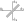
\includegraphics[width=0.5\linewidth, draft=false]{introduction/beamsplitter}
\caption{\label{fig:intro_beamsplitter} The beamsplitter transforms $\hat{a}_1, \hat{a}_2$ into $\hat{a}_3$, $\hat{a}_4$ via the matrix equation~\ref{eqn:intro_beamsplitter}.}
\end{figure}


The beamsplitter transformation which we will make use of in this Thesis is
\begin{equation}\label{eqn:intro_beamsplitter}
\pmqty{\hat{a}_3 \\ \hat{a}_4} = \pmqty{\tau & -\rho \\  \rho & \tau} \pmqty{\hat{a}_1 \\ \hat{a}_2},
\end{equation}
which transforms two input modes into two output modes as
\begin{equation}
\hat{a}_3 = \tau \hat{a}_1 - \rho \hat{a}_2 \qq{and} \hat{a}_4 = \rho \hat{a}_1 + \tau \hat{a}_2.
\end{equation}

\noindent To conserve energy we require $\tau^2 + \rho^2 = 1$, and since we have assumed that both $\tau$ and $\rho$ are real. %TODO: for the viva, make sure that I can justify this and say what effect it will have.
Finally, we will make extensive use of the following relation, which describes the output state when two input Fock states interfere on the beamsplitter. As in Ref.~\cite{Leonhardt2010} we take $\tau$ and $\rho$ to be real, such that $\tau = \sqrt{T}$ and $\rho = \sqrt{1-T}$, with $0 \le T \le 1$. The two-mode output state is:

\begin{align}\label{eqn:intro_beamsplitter_fock}
&\ket{n_1, n_2}^\prime  = \frac{1}{\sqrt{n_1! n_2!}} \sum_{k_1, k_2=0}^{n_1, n_2} \pmqty{n_1 \\ k_1} \pmqty{n_2 \\ k_2} \left(\sqrt{T}\right)^{k_1} \left(\sqrt{1-T}\right)^{n_1 - k_1} \left(-\sqrt{1-T}\right)^{k_2} \notag \\
%
&\left(\sqrt{T}\right)^{n_2 - k_2} \sqrt{\left(k_1 + k_2\right)! \left(n_1 + n_2 - k_1 - k_2\right)!} \times \ket{k_1 + k_2, n_1 + n_2 - k_1 - k_2}.
\end{align}
We later identify $T$ with channel transmission.



\FloatBarrier
\subsection{Master equation}

We now introduce some formalisms which will account for dynamics of a quantum system described by density matrix $\rho$. In a closed system, in which $\rho$ is a (potentially large) density matrix describing all degrees of freedom, the evolution is entirely governed by the von Neumann equation\footnote{$\hbar = 1$}

\begin{equation}
\ddt \rho = - i \left[\hat{H}, \rho \right],
\end{equation}

\noindent with $\hat{H}$ the Hamiltonian which controls the time-evolution of $\rho$. Although exact, the von Neumann equation is often difficult to solve, especially in the case of very large $\rho$.

There are many instances, however, where we do not care about modelling precise evolution of all degrees of freedom of $\rho$. One may think, perhaps, of a few quantum modes of interest which are weakly coupled to many more modes. We denote the interesting modes as ``system'' and the uninteresting ones as ``reservoir'', and write $\rho_S = \tr_R\left[\rho\right]$. In this case, instead of solving the von Neumann equation we can model the evolution of $\rho_S$ using the Lindblad master equation:

\begin{equation}\label{eqn:intro_lindblad}
\ddt \rho_S = - i \left[ \hat{H}_S, \rho_S \right] + \gamma \mathcal{L}\left[\hat{A}\right] \rho_S,
\end{equation}
where $\hat{H}_S$ describes evolution of the system state only, $\gamma$ is the decay rate of $\rho_S$ into the reservoir, and 
\begin{equation}
\mathcal{L}\left[\hat{A}\right] \rho_S = \hat{A} \rho_S \hat{A}^\dagger - \frac{1}{2} \hat{A}^\dagger \hat{A} \rho_S - \frac{1}{2} \rho_S \hat{A}^\dagger \hat{A}
\end{equation}
describes decay of $\rho_S$ into the reservoir. The term $\mathcal{L}\left[\hat{A}\right]$ is known as the Lindbladian, and $\hat{A}$ is the collapse operator which describes decay into the reservoir. The first term in Eq.~\ref{eqn:intro_lindblad} describes unitary (reversible) evolution of $\rho_S$, while the second term describes dissipative (irreversible) evolution.

We will make use of the Lindblad master equation with several different collapse operators in Chapter~\ref{chapter:phog}. For derivation of the master equation, including a detailed accounting of the requisite assumptions, we refer the reader to Refs.~\cite{Breuer2002, Carmichael1999}.



\FloatBarrier
\section{Quantum measurement}
We define a set of measurement operators $\left\{\hat{M}_j\right\}$ which act on a quantum state $\ket{\psi}$, each measurement operator corresponding to a different possible measurement outcome $j$. The probability that $j$ is observed after measurement on $\ket{\psi}$ is given by the overlap
\begin{equation}
\text{P}\left(j\right) = \bra{\psi}\hat{M}^\dagger_j \hat{M}_j\ket{\psi},
\end{equation}
while the state immediately after measuring $j$ is 
\begin{equation}
\ket{\psi^\prime} = \frac{\hat{M}_j \ket{\psi}}{\sqrt{\text{P}\left(j\right)}}.
\end{equation}
The set $\left\{\hat{M}_j\right\}$ should allow for any possible outcome $j$, and so we require
\begin{equation}
\sum_j \hat{M}_j^\dagger \hat{M}_j = \mathds{1},
\end{equation}
which encodes the normalization requirement for the probability distribution
\begin{equation}
\sum_j \text{P}\left(j\right) = 1.
\end{equation}

Let us identify $\hat{M}_j^\dagger \hat{M}_j$ with an operator $hat{E}_j$, which we shall refer to as a ``POVM" element. The set $\left\{\hat{E}_j\right\}$ is known as a ``POVM''\footnote{Which stands for \emph{positive operator valued measure}, for historical reasons.} \cite{Nielsen2010}. The POVM measurement formalism allows for a convenient description of quantum measurement statistics, as
\begin{equation}
\text{P}\left(j\right) = \langle\psi|\hat{E}_j|\psi\rangle
\end{equation}
with no reference to the post-measurement state. 

To illustrate the advantage of the POVM formalism, let us briefly consider an example, which we will revisit in later chapters. Suppose that Alice sends Bob one of two quantum states, either $\ket{\psi_1} = \ket{0}$ or $\ket{\psi_2} = \left(\alpha \ket{0} + \beta \ket{1}\right)$, with $\alpha^2 + \beta^2 = 1$. We assume that $\alpha, \beta \in \mathbb{R}$ for simplicity. Bob wishes to perform some measurement on his received state to determine whether he received $\ket{\psi_1}$ or $\ket{\psi_2}$. To do so, let Bob construct the following POVM:

\begin{align*}
\hat{E}_1 &:= \frac{\sqrt{2}}{\alpha + \sqrt{2}}\ket{1}\bra{1} \\
\hat{E}_2 &:= \frac{\sqrt{2} \alpha^2}{\left(\sqrt{2} + \alpha\right)\left(\alpha^2 + \beta^2\right)}\left(- \frac{\beta}{\alpha}\ket{0} + \ket{1}\right)\left(- \frac{\beta}{\alpha} \bra{0} + \bra{1}\right) \\
\hat{E}_3 &:= \mathds{1} - \hat{E}_1 - \hat{E}_2.
\end{align*}

\noindent One can readily check that if Bob performs $\left\{\hat{E}_1, \hat{E}_2, \hat{E}_3\right\}$ on state $\ket{\psi_1}$, there is zero chance he will record outcome $E_1$. Therefore, if Bob receives outcome $E_1$ he knows with certainty that Alice sent him $\ket{\psi_2}$. Likewise, if Bob receives outcome $E_2$ then he knows with certainty that Alice sent $\ket{\psi_1}$. However, should Bob receive $E_3$ then he gains no information about the state which Alice sent.

The POVM $\left\{\hat{E}_1, \hat{E}_2, \hat{E}_3\right\}$ thus performs an \emph{unambiguous discrimination} between the non-orthogonal states $\ket{\psi_1}$ and $\ket{\psi_2}$, and Bob will never misidentify the state which Alice sent. This comes at a cost: sometimes Bob gains no information at all. Designing POVMs and measurement schemes to optimally distinguish between a known set of states is a difficult problem which has received considerable attention over the years. We will revisit this question in Chapters~\ref{chapter:qds} and \ref{chapter:qss} in the context of quantum cryptography, where bounding a malicious party's ability to distinguish between quantum states is of critical importance.


\FloatBarrier
\subsection{Homodyne measurement}\label{sec:intro_homodyne}
Homodyne measurement is a frequently used technique for measuring the quadrature components of the quantum state. A homodyne detection scheme consists in measurement of quadrature operator $\hat{q}_\theta = \cos\theta \hat{q} + \sin\theta \hat{p}$, which gives outcome probabilities
\begin{equation}
\text{P}\left(q_\theta\right) = \ev{\rho}{q_\theta}
\end{equation}
where $\ket{q_\theta}$ is the eigenstate of $\hat{q}_\theta$ (c.f. Eq.~\ref{eqn:intro_quadrature_state}).% A homodyne measurement must specify the quadrature $\hat{q}_\theta$ which is being measured, then 
The set of operators $\dyad{q_\theta}$ form the homodyne POVM.

%Without loss of generality, consider just the position ($q$) and momentum ($p$) outcomes. The probability distributions $\text{P}\left(q\right), \text{P}\left(p\right)$ of homodyne measurement outcomes of state $\rho$ are equivalently given by marginal integrals of the Wigner function corresponding to $\rho$, over the conjugate quadrature:
%\begin{equation}
%\text{P}\left(q\right) = \int\limits_{-\infty}^\infty \mathrm{d}p \; W_\rho\left(q, p\right) \qq{and} \text{P}\left(p\right) = \int\limits_{-\infty}^\infty \mathrm{d}q \; W_\rho\left(q, p\right).
%\end{equation}

In practice the homodyne POVM is realised by mixing $\rho$ with a strong coherent state $\ket{\alpha}$, $\left|\alpha\right| \gg 1$ (the so-called ``local oscillator''), on a balanced ($50/50$) beamsplitter, and subtracting the measured photocurrents at output arm from each other. We depict this process in Fig.~\ref{fig:intro_homodyne}. We assume in the ideal case that the photocurrents $I_1$ and $I_2$ are such that
\begin{equation}
I_1 \propto \hat{n}_1 \qq{and} I_2 \propto \hat{n}_2 \qq{with} \hat{n}_i = \hat{a}_i^\dagger \hat{a}_i,
\end{equation}
and that the local oscillator may be treated classically, so
\begin{equation}
\hat{a}_1 = \frac{1}{\sqrt{2}} \left(\hat{a} - \alpha_{LO}\right) \qq{and} \hat{a}_2 = \frac{1}{\sqrt{2}}\left(\hat{a} + \alpha_{LO}\right).
\end{equation}
Then the difference in photocurrents $I_2 - I_1$ is
\begin{equation}
I_2 - I_1 \sim \hat{n}_2 - \hat{n}_1 = \alpha_{LO}^* \hat{a} + \alpha_{LO}\hat{a},
\end{equation}
and so
\begin{equation}
I_2 - I_1 \sim \sqrt{2} \left|\alpha_{LO}\right| \hat{q}_\theta,
\end{equation}
where $\theta$ is the phase of the local oscillator $\ket{\alpha}$. Varying the phase $\theta$ thus allows any general quadrature $\hat{q}_\theta$ of $\rho$ to be measured. The prefactor $\sqrt{2}\left|\alpha_{LO}\right|$ does not affect our measurement, and may be taken into account by an appropriate rescaling of measurement outcomes. A more realistic treatment of homodyne detection, including discussion of the range of validity of the above expressions, may be found in Refs.~\cite{Leonhardt1998, Serafini2017}.


\begin{figure}[htp]
\centering
\captionsetup{width=0.8\linewidth}
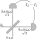
\includegraphics[draft=false, width=0.5\linewidth]{introduction/homodyne}
\caption{\label{fig:intro_homodyne} The homodyne detector mixes the mode to be measured, $\hat{a}_1$, with a strong local oscillator. The photocurrents are measured and subtracted $I_2 - I_1$, which gives measurement information about $\hat{q}_\theta$. The quadrature angle $\theta$ is controlled via the relative phase of the local oscillator.}
\end{figure}



\FloatBarrier
\subsection{Heterodyne measurement}\label{sec:intro_heterodyne}
A heterodyne measurement scheme corresponds to the POVM
\begin{equation}\label{eqn:intro_heterodyne_povm}
\hat{\mathds{1}} = \frac{1}{\pi} \int\limits_{\alpha \in \mathbb{C}} \Diff2 \alpha \; \dyad{\alpha}.
\end{equation}
The measurement gives outcome $\alpha$ with probability $(1/\pi)\ev{\rho}{\alpha}$. This scheme may be realised as a ``double-homodyne'' protocol, in which an input state $\rho$ is split on a balanced beamsplitter, and conjugate quadratures $\hat{q}_1$, $\hat{p}_2$ are measured on different output arms. Since they operate on different modes, the operators $\hat{q}_1$, $\hat{p}_2$ must commute. Simultaneous measurement of conjugate quadratures on the \emph{same} mode cannot be performed with arbitrary accuracy, and so the heterodyne measurement outcomes must pay the penalty of increased variance in $\text{P}\left(q\right)$, $\text{P}\left(p\right)$. Physically this arises from mixing with $\rho$ with vacuum on the first beamsplitter.


The heterodyne detector allows us to consistently define a joint probability distribution of the measurement outcomes $q_1$, $p_2$. This function is known as the Hussimi $Q$ function and is a well-defined probability distribution on the phase space\footnote{Unlike others such as Wigner function or $P$ function, which we refer to only as \emph{quasi}-probability distributions}. The Hussimi function corresponding to $\rho$ is thus
\begin{equation}
Q\left(q, p\right) = \frac{1}{\pi} \ev{\rho}{\alpha} \qq{with} \alpha = \frac{q + i p}{\sqrt{2}}.
\end{equation}

\noindent In the main body of the Thesis we will speak of the heterodyne measurement as effectively giving two outcomes, $\qout, \pout$, one from each homodyned arm. The $\alpha$ required for Eq.~\ref{eqn:intro_heterodyne_povm} are then given by $\alpha = \left(\qout + i \pout\right)/\sqrt{2}$.





\FloatBarrier
\section{Entropy and probability}
We will introduce and discuss some quantum entropies which are used in the first part of this Thesis. Quantum entropies are a marvellous and interesting area of quantum information theory, and there are many interesting similarities with and departures from classical information theory. Below we summarise some of the key results which we will make use of in this Thesis, and the reader is referred to Refs.~\cite{Nielsen2010, Tomamichel2016, Wilde2013, Watrous2018} for further information.



\FloatBarrier
\subsection{Conditional probabilities}
Let $X$ and $Y$ denote random variables, with their associated probability distributions $\text{P}\left(X\right), \text{P}\left(Y\right)$. The conditional probability of $X$ given $Y$, $\text{P}\left(X \given Y\right)$ measures the probability of event $X$, given prior knowledge of event $Y$. The probabilities $\text{P}\left(X\right)$, $\text{P}\left(Y\right)$ are known as the marginal probabilities, and are related to the conditional probability by summing over values of the prior $Y$:

\begin{equation}
\text{P}\left(X\right) = \sum_{Y=y} \text{P}\left(X \given Y=y\right) \text{P}\left(Y=y\right).
\end{equation}

\noindent Bayes' theorem may be used to relate conditional probabilities to each other:

\begin{equation}\label{eqn:intro_bayes}
\text{P}\left(X \given Y\right) = \text{P}\left(Y \given X\right) \frac{\text{P}\left(X\right)}{\text{P}\left(Y\right)},
\end{equation}

\noindent and we make extensive use of this formula in the first part of this Thesis.

\FloatBarrier
\subsection{Hoeffding's inequalities}
Let $\mathcal{X} = X_1, X_2, \dots, X_n$ be $n$ independent binary random variables. Let $\bar{\mathcal{X}}$ be their empirical mean and let $\mathbb{E}\left(\bar{\mathcal{X}}\right)$ be its expected value. Then $\forall \epsilon \ge 0$ we may bound the probability that the empirical mean $\bar{\mathcal{X}}$ differs from its expectation $\mathbb{E}\left(\bar{\mathcal{X}}\right)$ by the following inequalities:

\begin{align}
\label{eqn:hoeffding1}
\text{P}\left(\bar{\mathcal{X}} - \mathbb{E}\left(\bar{\mathcal{X}}\right) \ge \epsilon\right) &\le \text{exp}\left(- 2 \epsilon^2 n\right), \\
\label{eqn:hoeffding2}
\text{P}\left(\mathbb{E}\left(\bar{\mathcal{X}}\right) - \bar{\mathcal{X}} \ge \epsilon\right) &\le \text{exp}\left(- 2 \epsilon^2 n\right).
\end{align}



\noindent These inequalities are known as Hoeffding's inequalities \cite{Hoeffding1963} and will provide a necessary tool for analysis of our Quantum Digital Signatures protocol.



\FloatBarrier
\subsection{Shannon entropy}\label{sec:intro_shannon_entropy}
Let $X$ be a random variable, which takes values $X_1, X_2, \dots X_N$ with probability $\text{P}\left(X_1\right), \text{P}\left(X_2\right),\dots,\text{P}\left(X_N\right)$. The Shannon entropy associated with this variable is defined as 

\begin{equation}
H\left(X\right) = - \sum_{j=1}^N \text{P}\left(X_j\right) \log \text{P}\left(X_j\right).
\end{equation}

\noindent The Shannon entropy represents the degree of uncertainty which one possesses about the variable $X$. If the value of $X$ is known (minimum uncertainty) then\footnote{By convention we take $0 \log 0 = 0$.} $H\left(X\right) = 0$. Conversely, if all possible values of $X$ are equally likely (maximum uncertainty) then $H\left(X\right) = \log N$.

\FloatBarrier
\subsection{Binary entropy}
Let $X$ be a binary random variable, which takes value $0$ with probability $p$ and value $1$ with probability $1-p$. Then the binary entropy of $X$ is defined as

\begin{equation}\label{eqn:intro_binary_entropy}
\text{h}\left(X\right) = - x \log x - \left(1-x\right) \log \left(1-x\right).
\end{equation}
The binary entropy is a special case of the Shannon entropy for a binary random variable. We display the binary entropy $\text{h}\left(X\right)$ in Fig.~\ref{fig:binary_entropy}.

\begin{figure}[htp]
\centering
\captionsetup{width=0.8\linewidth}
\includegraphics[draft=false, width=0.7\linewidth]{introduction/binary_entropy}
\caption{\label{fig:binary_entropy} The binary entropy $\text{h}\left(x\right)$ is bounded by $\log 2$.}
\end{figure}


\FloatBarrier
\subsection{Mutual information}
We define the joint entropy $\text{H}\left(X, Y\right)$ of two random variables $X$ and $Y$ as the Shannon entropy of the joint probability distribution $\text{P}\left(X, Y\right)$. 

The conditional entropy of $X$, conditioned on $Y$, is
\begin{equation}\label{eqn:intro_definition_conditional_entropy}
\text{H}\left(X \given Y\right) = \text{H}\left(X, Y\right) - \text{H}\left(Y\right)
\end{equation}
which measures the average uncertainty we have about variable $X$ given that we know $Y$.

One may expand the conditional entropy as \cite{Wilde2013}
\begin{equation}\label{eqn:intro_conditional_entropy_expansion}
\text{H}\left(X \given Y\right) = \sum_{Y=y} \text{P}\left(Y=y\right) \text{H}\left( X \given Y=y \right),
\end{equation}
where the expansion is over particular outcomes of the prior variable. Equation~\ref{eqn:intro_conditional_entropy_expansion} admits a natural extension to the case when the prior variable is continuous rather than discrete, with $\sum_{y}$ replaced by $\int \mathrm{d}y$.


The mutual information between $X$ and $Y$ may be defined as

\begin{equation}\label{eqn:intro_mutual_information}
I\left(X : Y\right) = \text{H}\left(X\right) - \text{H}\left(X \given Y\right),
\end{equation}

\noindent which is a measure of how much knowledge of one variable reduces uncertainty about the other variable. The mutual information is symmetric in its arguments.


\FloatBarrier
\subsection{Von Neumann entropy}
The von Neumann entropy of a quantum state $\rho$ is
\begin{equation}
\text{S}\left(\rho\right) = - \tr\left[\rho \log \rho \right],
\end{equation}
which may be equivalently calculated as
\begin{equation}\label{eqn:intro_von_neumann}
\text{S}\left[\rho\right] = - \sum_j \lambda_j \log \lambda_j,
\end{equation}
where $\lambda_j$ are the eigenvalues of $\rho$. The von Neumann entropy is always non-negative, and is zero when $\rho$ is pure.

By analogy with the Shannon entropy we will additionally define the joint entropy of a composite system $\rho_{A, B}$ in the obvious way
\begin{equation}
\text{S}\left(\rho_{A, B}\right) = - \tr\left[\rho_{A, B} \log \rho_{A, B}\right].
\end{equation}

\noindent The conditional von Neumann entropy between quantum systems $A$ and $B$ may then be defined
\begin{equation}
\text{S}\left(A \given B\right) = \text{S}\left(A, B\right) - \text{S}\left(B\right),
\end{equation}
where the von Neumann entropy of a quantum system $A$ or $B$ should be understood as the entropy of the corresponding state $\rho_A$, $\rho_B$.


\FloatBarrier
\subsection{Holevo information}\label{sec:intro_holevo}
The Holevo information $\chi$ is an upper bound on the mutual information $I$, and plays a crucially important role in many areas of quantum information processing. 

We introduce two players, Alice and Bob. Let Alice prepare a state $\rho_j$, $j = 1, 2, \dots, N$, with probability $p_1, p_2, \dots, p_N$. Bob wishes to distinguish which of the $\rho_j$ Alice has prepared. 

Bob may perform any measurement described by POVM elements $\left\{E_K\right\}$, and he receives a measurement outcome $K$. Then the mutual information $I\left(j : K\right)$ describes the knowledge of which $\rho_j$ was prepared, given Bob's measurement outcome $K$. The mutual information is upper bounded by the Holevo information

\begin{equation}\label{eqn:intro_holevo_bound}
I\left(j : K \right) \le \chi \left(j : K \right),
\end{equation}
with the Holevo information $\chi$ defined as

\begin{equation}\label{eqn:intro_holevo}
\chi\left(j : K\right)  = \text{S}\left(\rho\right) - \sum_j p_j \text{S}\left(\rho_j\right),
\end{equation}
with
\begin{equation}
\rho = \sum_j p_j \rho_j.
\end{equation}

\noindent For a pleasing proof that $I$ is bounded by $\chi$ we refer the reader to Ref.~\cite{Nielsen2010}. 

Throughout this Thesis we will refer to the first term in Eq.~\ref{eqn:intro_holevo} as the \emph{a priori} entropy (with its corresponding \emph{a priori} state $\rho$), while we refer to the second term as the \emph{a  posteriori} entropy (with its corresponding \emph{a posteriori} state $\rho_j$). The bound in Eq.~\ref{eqn:intro_holevo_bound} will be used extensively in the cryptographic security proofs in the first part of this Thesis.


\FloatBarrier
\subsection{Conditioning cannot increase entropy}

A useful property of both Shannon and von Neumann entropies is that ``conditioning cannot increase entropy.'' This directly encodes the intuition that gaining more information about a system cannot lead to increased uncertainty - at worst it will leave the uncertainty in our knowledge unchanged. Quantitatively, we have for a quantum state $\rho_{A, B}$

\begin{equation}
\text{S}\left(A\right) \ge \text{S}\left( A \given B \right),
\end{equation}
where the entropy of system $A$ should be understood as the entropy of $\rho_A = \tr_B\left[\rho_{A, B}\right]$. Similarly, for classical random variables $X, Y$:
\begin{equation}
\text{H}\left(X\right) \ge \text{H}\left(X \given Y\right).
\end{equation}


\FloatBarrier
\subsection{Chain rule for conditional Shannon entropy}

Let $X_1, \dots, X_n$ and $Y$ be random variables. Then \cite{Nielsen2010, Wilde2013}
\begin{equation}\label{eqn:intro_chain_rule}
\text{H}\left(X_1, \dots, X_n \given Y\right) = \sum_{i=1}^n \text{H}\left(X_i \given Y, X_1, \dots, X_{i-1}\right).
\end{equation}

\noindent This property is known as the conditional Shannon entropy \emph{chain rule} and is readily proven by induction (see e.g. Ref.~\cite{Nielsen2010}) using Eq.~\ref{eqn:intro_definition_conditional_entropy}.

\FloatBarrier
\section{Summary}
\MT{Add a quick summary sentence to ensure that the chapter does not have such an abrupt stop.}



In this chapter we have provided a brief overview of several key concepts and tools which underpin this Thesis. Additional material which is required will be introduced as it is used. We have introduced the density matrix formalism and discussed how it relates to other methods for describing quantum states of light, such as the Wigner function and the covariance matrix. Although in this Thesis we work primarily in terms of the density matrix, the Wigner function has provided us with a useful visualization tool in this Chapter. Furthermore, the Wigner function simplifies calculations in Appendix~\ref{appendix:noisy_perr} which are in principle possible, but difficult in general, using density matrices. The covariance matrix is another useful tool which warrants extensive study in its own right. We use the covariance matrix only in Chapter~\ref{chapter:phog} to measure the Gaussian entanglement properties of a state. The Wigner function representation for a multimode quantum state is intertwined with the covariance matrix description, and we refer the reader to Ref.~\cite{Serafini2017} for an excellent discussion of how to move between the two pictures.

In the first half of this Thesis, Chapters~\ref{chapter:qds}-\ref{chapter:aqc}, we will use the density matrix description, along with the beamsplitter relation for input fock states in order to model the passage of a quantum state through a channel. In the cryptographic protocols discussed there, a malevolent party is assumed to replace the channel with an ideal beamsplitter, and they have control over the second input port, and receive the reflected output state. We model this interaction, and then use the entropies introduced above to bound the ability of a dishonest player to break the protocol.

In the second half of this Thesis we will examine in depth the dynamics of a coherent state in several different scenarios. Our key tool here will be the Lindblad equation which describes the evolution of our density matrix. When possible we draw conclusions analytically, but our main techniques will be the numerical methods discussed at length in Appendix~\ref{appendix:phog_numerical_methods}. These allow us to gain an understanding of the state evolution, sometimes even if computational constraints prevent us from accessing the full density matrix. 






